% !TEX root = slides.tex
%%%%%%%%%%%%%%%%%%%%%%%%%%%%%%%%%%%%%%%%%%%%%%%%%%%%%%%%%%%%%%%%%%%%%%%%%%%%%%
\begin{frame}[t]
\label{bayes}
\frametitle{Bayes formula for Parameter Inference}
\bi
\item Collected data: \qquad $\{(x_i,y_i)\}_{i=1}^N$
\item Data model: \qquad $y_i=f(x_i;\lambda) + \epsilon_i$
\item Bayes formula:\vspace*{-2mm}
\ben
\mathop{
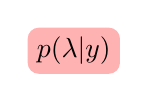
\begin{tikzpicture} \node [rounded corners,fill=red!30] {$\displaystyle p(\lambda|y)$}; \end{tikzpicture}
}_{\textrm{\color{blue}Posterior}}
= \frac{
\stackrel{\small\textrm{\color{blue}Likelihood}}
{
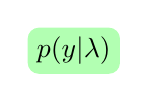
\begin{tikzpicture} \node [rounded corners,fill=green!30] {$\displaystyle p(y|\lambda) $}; \end{tikzpicture}
}
\,\,
\stackrel{\small\textrm{\color{blue}Prior}}
{
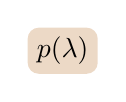
\begin{tikzpicture} \node [rounded corners,fill=brown!30] {$\displaystyle p(\lambda) $}; \end{tikzpicture}
}
} {
\overbracket[0pt]{
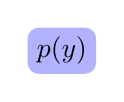
\begin{tikzpicture} \node [rounded corners,fill=blue!30] {$\displaystyle p(y) $}; \end{tikzpicture}
}_{\textrm{\color{blue}Evidence}}
}
\een
\bigskip
\item Prior: knowledge of $\lambda$ prior to data
\item Likelihood: forward model and measurement noise
\item Posterior: combines information from prior and data
\item Evidence: normalizing constant for present context
\ei

\end{frame}
%%%%%%%%%%%%%%%%%%%%%%%%%%%%%%%%%%%%%%%%%%%%%%%%%%%%%%%%%%%%%%%%%%%%%%%%%%%%%%
